\documentclass[10pt]{article}
\usepackage[margin=1 in, letterpaper]{geometry}
\usepackage{fontspec, graphicx, amsmath, amssymb, amsthm, array, physics, enumitem, cancel, multicol, float}
\usepackage{latexsym, marvosym}
\usepackage[dvipsnames]{xcolor}

\setmainfont{Linux Libertine O}
\setsansfont{Linux Biolinum O}
\setmonofont{Latin Modern Mono}
\setmathrm{Latin Modern Math}
\theoremstyle{definition}
\newtheorem{theo}{\color{Maroon} Theorem}[section] 
\newtheorem{defin}[theo]{\color{Maroon} Definition}
\newtheorem{example}[theo]{\color{Maroon} Example}
\newtheorem{prob}[theo]{\color{Maroon} Problem}
% \newtheorem{example}[section]{\color{Maroon} Example}

\theoremstyle{remark}
\newtheorem*{soln}{\color{Maroon} Solution}

\newcommand{\R}{\mathbb{R}}
\newcommand{\Q}{\mathbb{Q}}
\newcommand{\Z}{\mathbb{Z}}
\newcommand{\N}{\mathbb{N}}

%%%%%%%%%%%%%%%%%%% Statistics %%%%%%%%%%%%%%%%%%%%
\newcommand{\E}[1]{\mathbb{E}\left[ #1 \right]}
\newcommand{\Prob}[1]{\mathbb{P}\left[ #1 \right]}
\newcommand{\cov}[2]{\textnormal{Cov}\left[ #1, #2 \right]}
\renewcommand{\var}[1]{\textnormal{Var}\left[ #1 \right]}
\newcommand{\Unif}{\textnormal{Unif}}
\newcommand{\Norm}{\mathcal{N}}

%%%%%%%%%%%%%%%%%%%%%%%%%%%%%%%%%%%%%%%%%%%%%%%%%%%%%%%%%%%%%%%%%%%%
\newcommand{\inserttitle}{Section 02}
\newcommand{\insertauthor}{Max Guo \& Seung Hwan An}
\newcommand{\insertcourse}{STAT 110}
%%%%%%%%%%%%%%%%%%%%%%%%%%%%%%%%%%%%%%%%%%%%%%%%%%%%%%%%%%%%%%%%%%%%

\usepackage{fancyhdr}
\setlength{\headheight}{15pt}
\pagestyle{fancy}
\fancyhf{}
\fancyhead[C]{\thepage}
\fancyhead[L]{\inserttitle}
\fancyhead[R]{\insertauthor}

%%%%%%%%%%%%%%%%%%%%%%%%%%%%%%%%%%%%%%%%%%%%%%%%%%%%%%%%%%%%%%%%%%%%

\begin{document}

{\noindent\Huge\bf  \\[0.1\baselineskip] {\inserttitle }}\\[2\baselineskip]
{{\bf \insertcourse}\\ {\textit{September 13, 2021}}} \hfill {\large \textsc{\insertauthor}}
\smallskip

\hfill \noindent \textit{Credits to Vincent Li and Dylan Li}

\section{Disjointness Versus Independence Versus Conditional Independence}

	\begin{description}
		\item[Disjoint Events] - $A$ and $B$ are disjoint when they cannot happen simultaneously, or
		  \begin{align*}
			P(A \cap B) &= 0\\
			A \cap B &= \emptyset
		  \end{align*}
		\item[Independent Events] - $A$ and $B$ are independent if knowing one gives you no information about the other. $A$ and $B$ are independent if and only if one of the following equivalent statements hold: 
		   \begin{align*} 
			P(A\cap B) &= P(A)P(B) \\
			P(A|B) &= P(A)
		   \end{align*}
		\item[Conditional Independence] - $A$ and $B$ are conditionally independent given ${\bf C}$ if: $P(A\cap B|C) = P(A|C)P(B|C)$. Conditional independence does not imply independence, and independence does not imply conditional independence.
	\end{description}
	
	\Biohazard \ It is important to note that any one of these do NOT imply another! Give an example of: 
	\begin{itemize}
	    \item Disjoint events that are \textit{not} independent. 
	    
	   % \vspace{0.7 in} 
	    
	    \fbox{\parbox{0.9 \textwidth}{Let $H$ be the event that I get heads on a coin flip and $T$ be the event that I get tails. $H$ and $T$ are disjoint, but clearly \textit{as dependent as they can be}.}}
	    
	    \item Independent events that are \textit{not} disjoint. 
	    
	   % \vspace{0.7 in} 
	    
	    \fbox{\parbox{0.9 \textwidth}{Let $H_1$ be the event I get heads on first coin flip and $H_2$ that I get heads on second coin flip. $H_1$ and $H_2$ are independent, so $P(H_1 \cap H_2) = P(H_1) P(H_2) = 1/4$, and thus not disjoint.}}
	    
	    \item Independent events that are \textit{not} conditionally independent.
	    
	   % \vspace{0.7 in} 
	    
	    \fbox{\parbox{0.9 \textwidth}{Let $H_1$ be the event that I get heads on first coin flip and $H_2$ that I get heads on second coin flip, and $O$ be the event that I get 1 head out of two coin flips. These are independent, but \textit{conditioning} on $O$, if $H_1$ happens, $H_2$ cannot happen, so they are \textit{not} conditionally independent on $O$.}}
	    
	    \item Conditionally independent events that are \textit{not} independent.
	    
	   % \vspace{0.7 in} 

        \fbox{\parbox{0.9 \textwidth}{Suppose we have one fair coin and one heavily biased coin. Let $H_1$ be the event that I get heads on first coin flip and $H_2$ that I get heads on second coin flip, and $O$ the event that I choose the fair coin. $H_1$ and $H_2$ are \textit{not} independent, since if I get heads on the first flip, we are much much more likely to have picked the biased coin, and thus much more likely to land on heads the next flip. However, conditional on either $O$ happening or not, this is just two coin flips, which are conditionally independent on $O$ or $O^c$. }}

    \end{itemize}
	
\pagebreak	
	
\section{Conditioning is the Soul of Statistics}

Before we start, we want to remind you that \textit{conditional probability is extremely counterintuitive}. There are a lot of results that just sounds wrong at first, but after careful reasoning, that you will be able to convince yourself is true. This, we think, is the least mathematically difficult, but by far the most conceptually difficult part of the course. 

	\begin{description}
		\item[Joint Probability] - $P(A \cap B) $ or $P(A, B)$ - Probability of $A$ \emph{and} $B$.
		\item[Marginal (Unconditional) Probability] - $P(A)$ - Probability of $A$
		\item[Conditional Probability] - $P(A|B)$ - Probability of $A$ given $B$ occurred.
		
		\Biohazard \ Note that in general $P(A|B) \neq P(B|A)$. 
		
		\item[Conditional Probability is Probability] - $P(A|B)$ is a probability as well, restricting the sample space to $B$ instead of $\Omega$. Any theorem that holds for probability also holds for conditional probability.
		\item[Bayes' Rule] - Bayes' Rule unites marginal, joint, and conditional probabilities. This is \emph{the most important concept of the week}, and one of the backbones of statistics. We use this as the definition of conditional probability.
	    $$ \boxed{ \underbrace{P(A|B)}_{\text{posterior}} = \frac{P(A \cap B)}{P(B)} = \underbrace{\frac{P(B|A)}{P(B)}}_{\text{update factor}} \underbrace{P(A)}_{\text{prior}} }$$
	    
	    We can consider Bayes' Rule as a mathematical description of how we should \textit{update} our belief about probability of some event happening ($A$) \textit{given} that we saw $B$ happen. 
	    
	    \fbox{\parbox{0.9 \textwidth}{A Bayesian believes that probability reflects the degree of belief I have of the event happening. Bayesian view of the world is information-theoretic, in that Bayesians have a precise formula for how one should update one's priors as information keeps streaming in.}}
	   
	    Since conditional probabilities \textit{are} probabilities, Bayes' rule still work with conditional probabilities:
	    
	    $$ P(A|B,C) = \frac{P(B|A,C)}{P(B|C)} P(A|C) $$
	    
	    \item[Intersection of Many Events] $$P( A_1 \cap A_2 \cap \ldots \cap A_n) = P(A_1) P(A_2 | A_1) P(A_3 | A_2, A_1) \ldots P(A_n | A_{n-1}, \ldots, A_1)$$
	   
	\end{description}

\begin{example} \textbf{(A girl born in winter)} This example is on page 49-52 of the textbook. Make sure to give this a thorough read, since it is an instructive example on how nuanced conditional probability is. A family has two children. Find the probability that both children are girls, given that at least one of the two is a girl.

\medskip 

$$P(\text{both girls}|\text{at least 1 girl}) = \frac{P(\text{both girls},\text{at least 1 girl})}{P(\text{at least 1 girl})} = \frac{P(\text{both girls})}{P(\text{at least 1 girl})} = \frac{1/4}{3/4} = \boxed{\frac{1}{3}}$$

\medskip 

A family has two children. Find the probability that both children are girls, given that at least one of the two is a girl who was born in winter. Assume that the four seasons are equally likely and that gender is independent of season.

\medskip

$$P(\text{both girls}|\text{at least 1 winter girl}) = \frac{P(\text{both girls},\text{at least 1 winter girl})}{P(\text{at least 1 winter girl})} $$ Probability of there being at least 1 winter girl can be gotten by considering its complement, the probability that there is no winter girl. Probability of being no winter girl is $(7/8)^2$, so the denominator is $1-(7/8)^2=15/64$. The numerator is \begin{align*}
    P(\text{both girls},\text{at least 1 winter girl}) & = P(\text{both girls},\text{at least 1 winter child}) \quad \text{ since we are guaranteed that child to be a girl}\\
    & = P(\text{both girls})P(\text{at least 1 winter child}) \quad \text{ due to independence} \\
    & = (1/4) (1- (3/4)^2) = 7/64
\end{align*}
Hence the answer is $7/15$! Note that this is now much closer to $1/2$ than our previous answer of $1/3$ when we are just given that one child is a girl! Why is that?

\vspace{1 in}

\end{example}
	
\section{Law of Total Probability}

\begin{figure}[H]\centering
	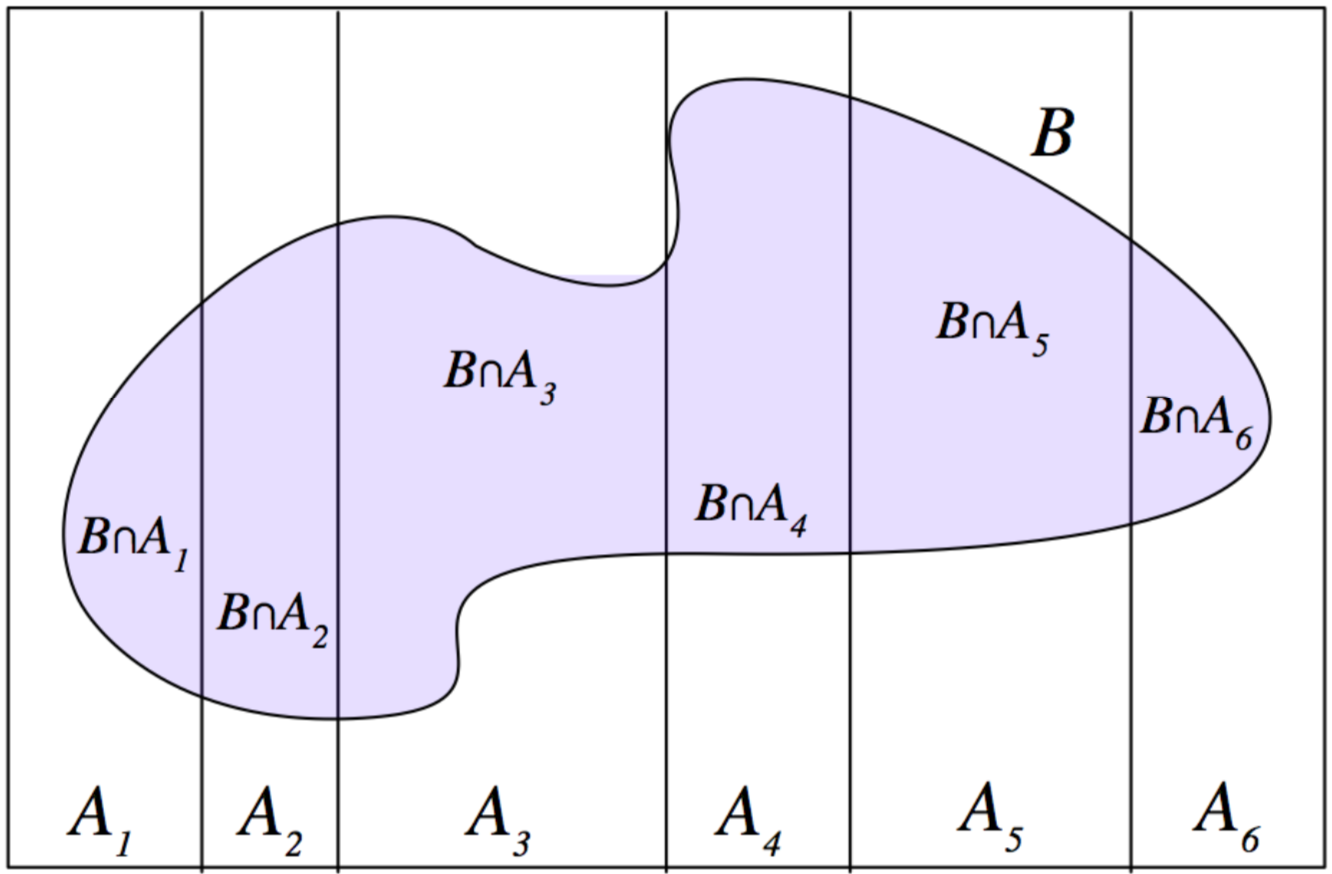
\includegraphics[width = 0.6\textwidth]{image/lotp.png}
	\caption{The $A_i$ partition the sample space. $P(B)$ is equal to $\sum_i P (B \cap A_i)$. Image from textbook.}
\end{figure}

This is a useful way to break up a harder problem into simpler pieces, conditioning on what we wish we knew. For any event $B$ and set of events $A_1, A_2, A_3, ... A_n$ that partition a space, the following are true:
   \begin{align*} 
        P(B) &= P(B | A_1)P(A_1) + P(B | A_2)P(A_2) + ...  P(B | A_n)P(A_n)\\
        P(B) &= P(B \cap A_1)+ P(B \cap A_2)+ ...  P(B \cap A_n)
   \end{align*} 
   or in the simplest case where $A$ is just any event
   \begin{align*} 
        P(B) &= P(B | A)P(A) + P(B | A^c)P(A^c) \\
        P(B) &= P(B \cap A)+ P(B \cap A^c)
   \end{align*} 

Again, since conditional probability is probability, we can extend this to: $$ P(B|C) = \sum_{i=1}^n P(B|A_i, C) P(A_i | C) $$

\pagebreak
\section{Practice Problems}

\begin{prob} \textbf{(The Flippant Juror)}. \ \ (Frederick Mosteller, \emph{Fifty Challenging Problems in Probability}) A three-man jury has two members each of whom independently has probability $p$ of making the correct decision and a third member who flips a coin for each decision (majority rules). A one-man jury has probability $p$ of making the correct decision. Which jury has the better probability of making the correct decision?

\end{prob}

% \vspace{1.5 in}

\fbox{\parbox{0.9 \textwidth}{Three-man jury can make the correct decision if:
\begin{itemize}
    \item First two members both make the correct decision. This happens with probability $p^2$.
    \item Only one of the first two members and third member make the correct decision. This happens with probability $2p(1-p) \times \frac{1}{2} = p-p^2$. 
\end{itemize}
Hence the three man jury make the correct decision with probability $p$, so exactly the same probability.}}

\begin{prob} \textbf{(Biased Coins)} \ \ Suppose that you have two coins. One of these coins is fair, meaning that it is heads with probability $1/2$, and the other is heads with probability $3/4$. 
\begin{enumerate}[label = (\alph*)]
	\item Let's say that you randomly select one of these two coins and you select each coin with probability 1/2. If you flip this randomly selected coin once, what is the probability that you flip a heads? What if you flip heads twice?
	
% 	\vspace{ 1 in}
	
	\fbox{\parbox{0.9 \textwidth}{Let $F$ be the event that I pick the fair coin. Then, $$P(H) = P(H|F)P(F) + P(H|F^c)P(F^c) = \frac{1}{2} \frac{1}{2} + \frac{3}{4} \frac{1}{2} = \frac{5}{8}$$ $$P(HH) = P(HH|F)P(F) + P(HH|F^c)P(F^c) = \left( \frac{1}{2} \right)^2 \frac{1}{2} + \left(\frac{3}{4}\right)^2 \frac{1}{2} = \frac{13}{32}$$}}
	
	\item You randomly select a coin and flipped it two times, obtaining heads each time. What is the probability that you randomly selected the fair coin?
	
% 	\vspace{ 1 in}
	
	\fbox{\parbox{0.9 \textwidth}{ By Bayes' rule, $$P(F | HH) = \frac{P(HH|F)}{P(HH)} P(F) = \frac{1/4}{13/32} \frac{1}{2} = \frac{4}{13}$$ }}
	
	\item Given this information, what is now the probability that if you flip the coin one more time, it will come up as heads?
	
	\fbox{\parbox{0.9 \textwidth}{ By LOTP, $$ P(H) = P( H|F) P(F) + P(H|F^c)P(F^c) = \frac{1}{2} \frac{4}{13} + \frac{3}{4} \frac{9}{13} = \frac{35}{52} $$ }}
	
\end{enumerate}
\end{prob}

\newpage
\begin{prob} \textbf{(Candies in a Jar)}. (Xinfeng Zhou, \emph{A Practical Guide to Quantitative Finance Interviews}) You remove candies one by one from a jar with 10 red candies, 20 blue candies, and 30 green candies. What is the probability that there are at least 1 blue candy and 1 green candy left in the jar when you have removed all the red candies? \footnote{Hint: Having at least 1 blue candy and 1 green candy left means that the last red candy must have been removed before the last blue and green candies in the 60-candy sequence. Try conditioning on the blue candy being the last in the 60-candy sequence, and conditioning on the green candy being the last in the 30-candy sequence (10 red, 20 green). What happens if the green candy is the last in the 60-candy sequence?}

\end{prob} 

% \vspace{2.5 in}

\fbox{\parbox{0.9 \textwidth}{  \begin{align*} \Pr[\text{1 blue and 1 green left}] &  = \Pr[\text{1 blue and 1 green left} | \text{blue last}] \Pr[\text{blue last}] \\ & \hspace{1 in} + \Pr[\text{1 blue and 1 green left} | \text{green last}] \Pr[\text{green last}] \\ & \hspace{1 in} + \Pr[\text{1 blue and 1 green left} | \text{red last}] \Pr[\text{red last}] \\ & = \Pr[ \text{green last among green/red} ] \cdot \frac{1}{3} + \Pr[ \text{blue last among blue/red} ] \cdot  \frac{1}{2} \\ & = \frac{3}{4} \frac{1}{3} + \frac{2}{3} \frac{1}{2} = \frac{7}{12} \end{align*} }}



\end{document}